\documentclass{article}
\usepackage[utf8]{inputenc}
\usepackage{hyperref}
\usepackage{listings}
\usepackage{graphicx}
\graphicspath{ {./Images/} }

\title{COMP390: Git Tutorial}
\author{Adrian Manhey}
\date{February 2022}

\begin{document}

\maketitle

\section{Introduction}

The purpose of this tutorial is to allow someone who has installed Git to understand how to use it. If you have not yet installed Git, you can follow the tutorial \href{https://git-scm.com/book/en/v2/Getting-Started-Installing-Git}{here} in order to do so.

\section{Git Overview}
First let's quickly go over the four data stores of Git. There are four parts in the Git life-cycle:

\begin{itemize}
    \item Working tree – files currently on your computer
    \item Staging area – files/changes ready to be committed
    \item Local repository – files (and their history) that have been committed
    \item Remote repository – files (and their history) on a different computer
\end{itemize}

\begin{center}
    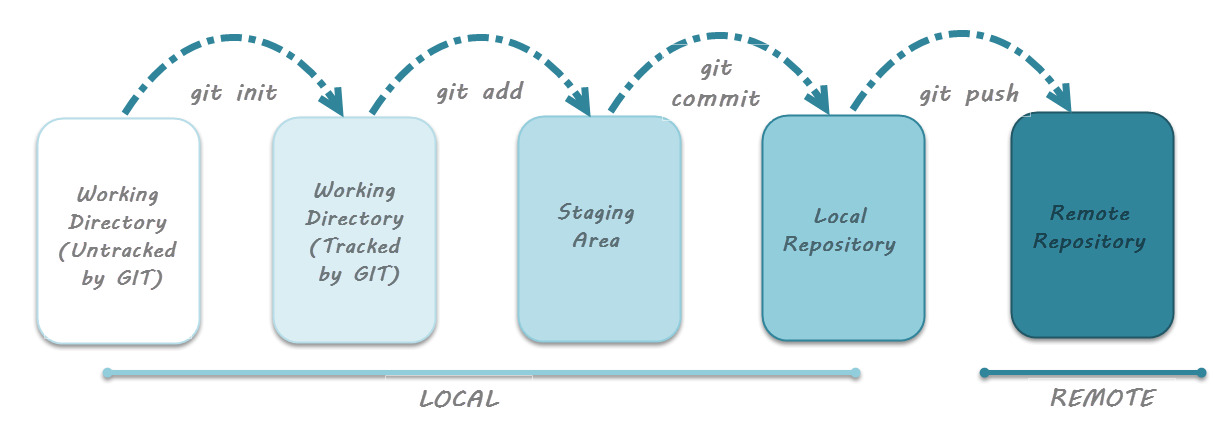
\includegraphics[width=8cm]{4 Git Life Cycle.png}
\end{center}

We will go over the commands that move documents from each stage later on this tutorial but have these components in mind as you follow along.
\section{Getting Started}

To begin we need a Git Repository, which can either be created on your local machine or cloned from an existing repository. If you wanted to clone an existing repository you would navigate to the directory you wanted the repository in via the command line and then use the command:

\begin{verbatim}
$ git clone <repository URL>
\end{verbatim}

However, in this tutorial we are going to create our own repository (repo). To begin navigate to the directory you want to create your repo in.
Once there, let's create a new README.md file for our repo.
One way to do this is using the "echo" command:

\begin{verbatim}
echo "# COMP390Tutorial" >> README.md
\end{verbatim}

This command saves the text in quotations in the README.md file on the last empty line. If we wanted to overwrite the file we would use a single ">" instead of two. This newly created file exists on the working tree. Now let's initialize the repository:

\begin{verbatim}
git init
\end{verbatim}

Now we have to begin tracking our files to save the changes that have been made. The "git add" command adds a file to the list of files we want to begin tracking, files need to be added anytime a set of changes have made to them that we want to save. This moves our file from the working tree to the staging area. Then the "git commit" command saves the changes locally and moves them from the staging area to the local repository.

\begin{verbatim}
git add README.md
git commit -m "first commit"
\end{verbatim}

Next we begin moving our file from the local repository to the remote repository. The "git branch" command tells git which branch we want to work on, since this is the only file so far it's going to be on the "main" branch. Then we link our local repo to the remote repo with the next command, so git knows where to save our file. Finally we push our files to the remote repo.
%Do we need to create the repo on github first?
\begin{verbatim}
git branch -M main
git remote add origin https://github.com/<GitHub username>/
    <repository name>.git
git push -u origin main
\end{verbatim}

\begin{center}
    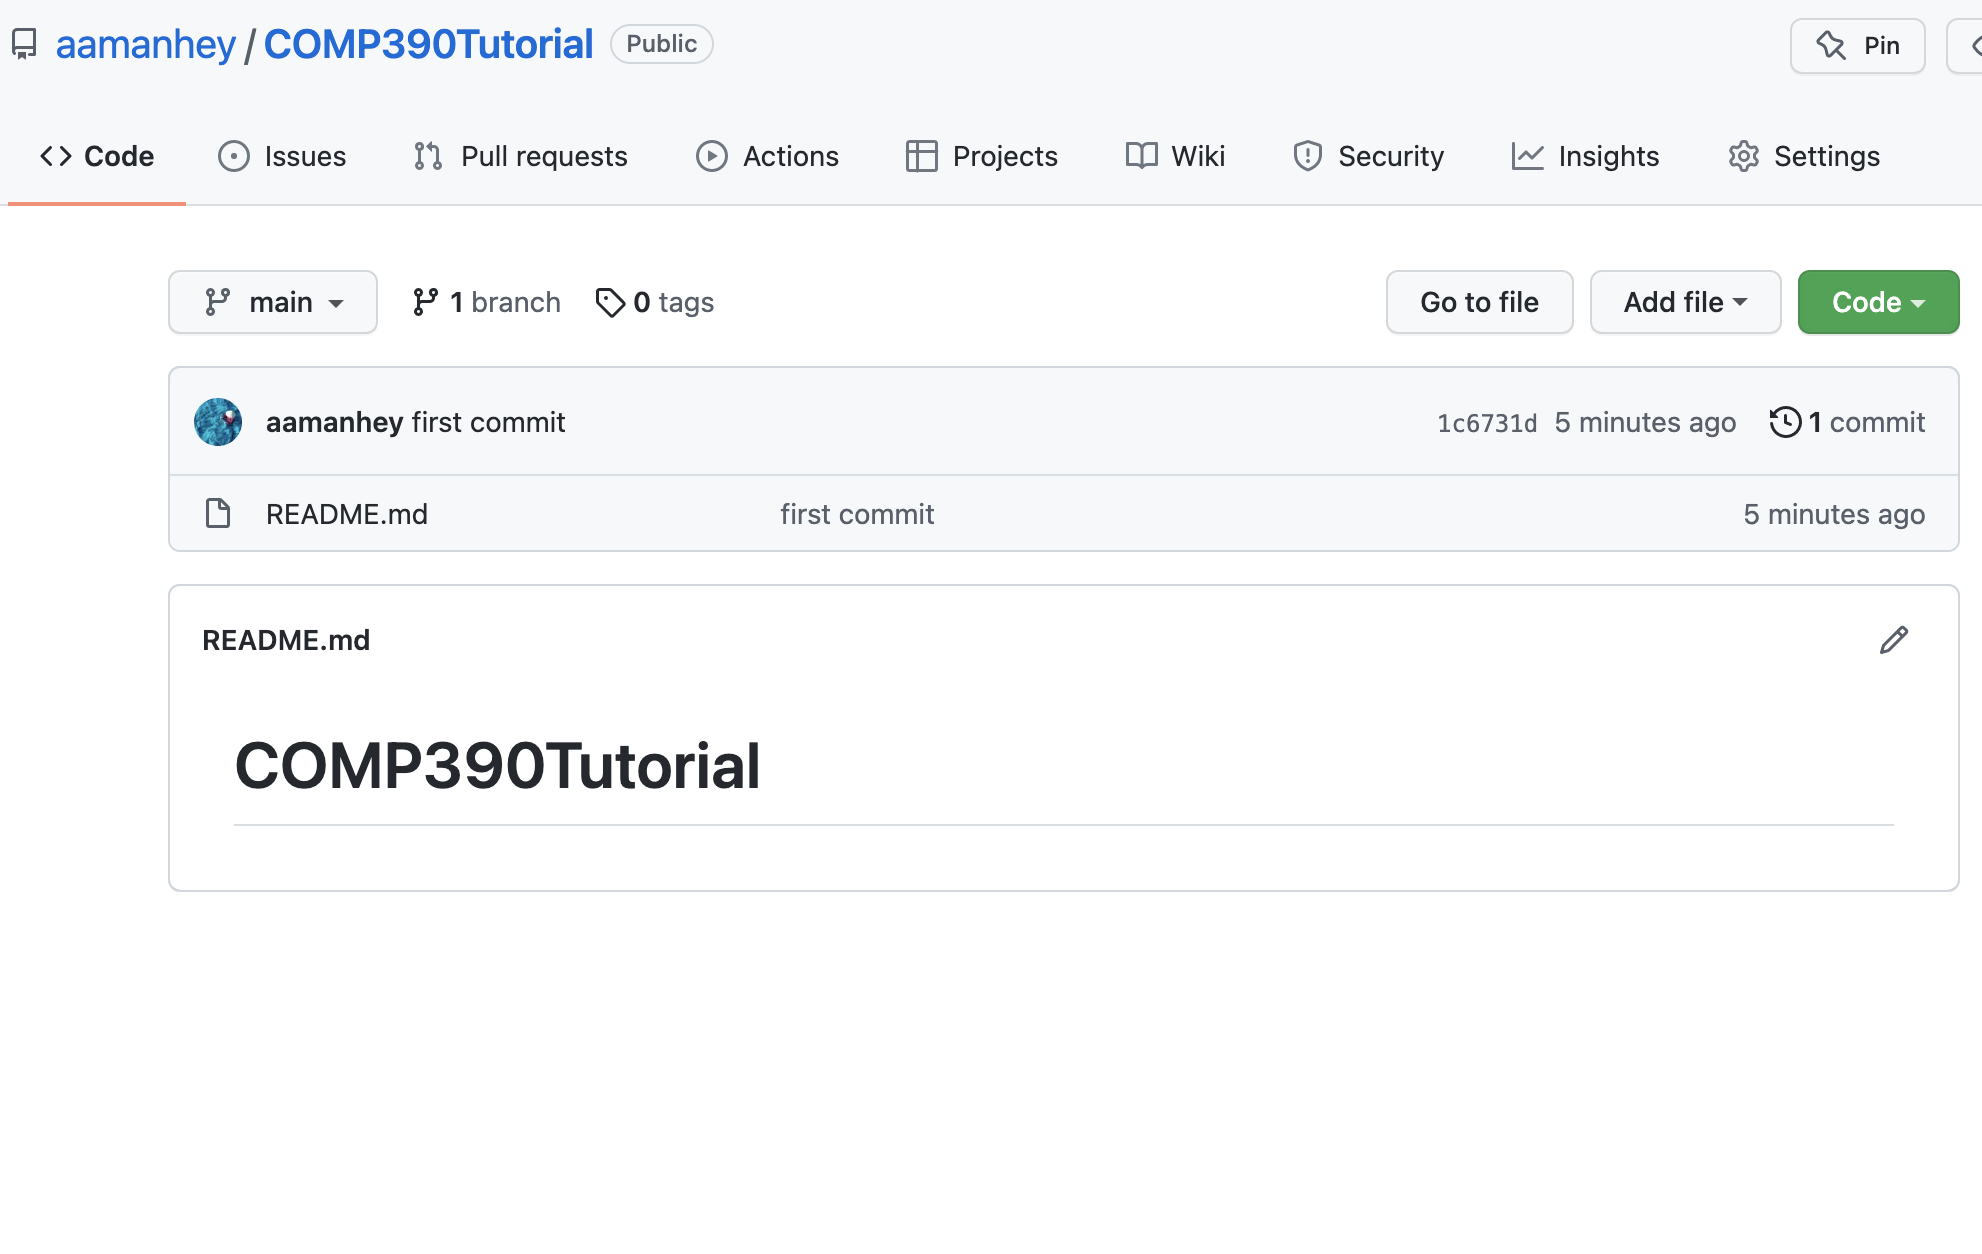
\includegraphics[width=8cm]{RepoReadme1.png}
\end{center}

Now that our files are in the remote repo we can view them on \href{https://github.com/}{GitHub} by navigating to your repo.
You should see a "README.md" file with "COMP390 Tutorial" inside.

\section{Changing Files}

Let's make some changes! First let's add onto our current README file and then create an outline.txt file to document our project.

\begin{verbatim}
echo "Additional info about our project." >> README.md
echo "Project Outline" > outline.txt
\end{verbatim}

If we wanted to move both of them to the staging area we could use the "A" tag with the add command but let's just add the README file.

\begin{verbatim}
git add README.md
\end{verbatim}

To check to see which files have been changed we can use the following command \begin{verbatim}
    git status
\end{verbatim}

This should return something similar to this:

\begin{center}
    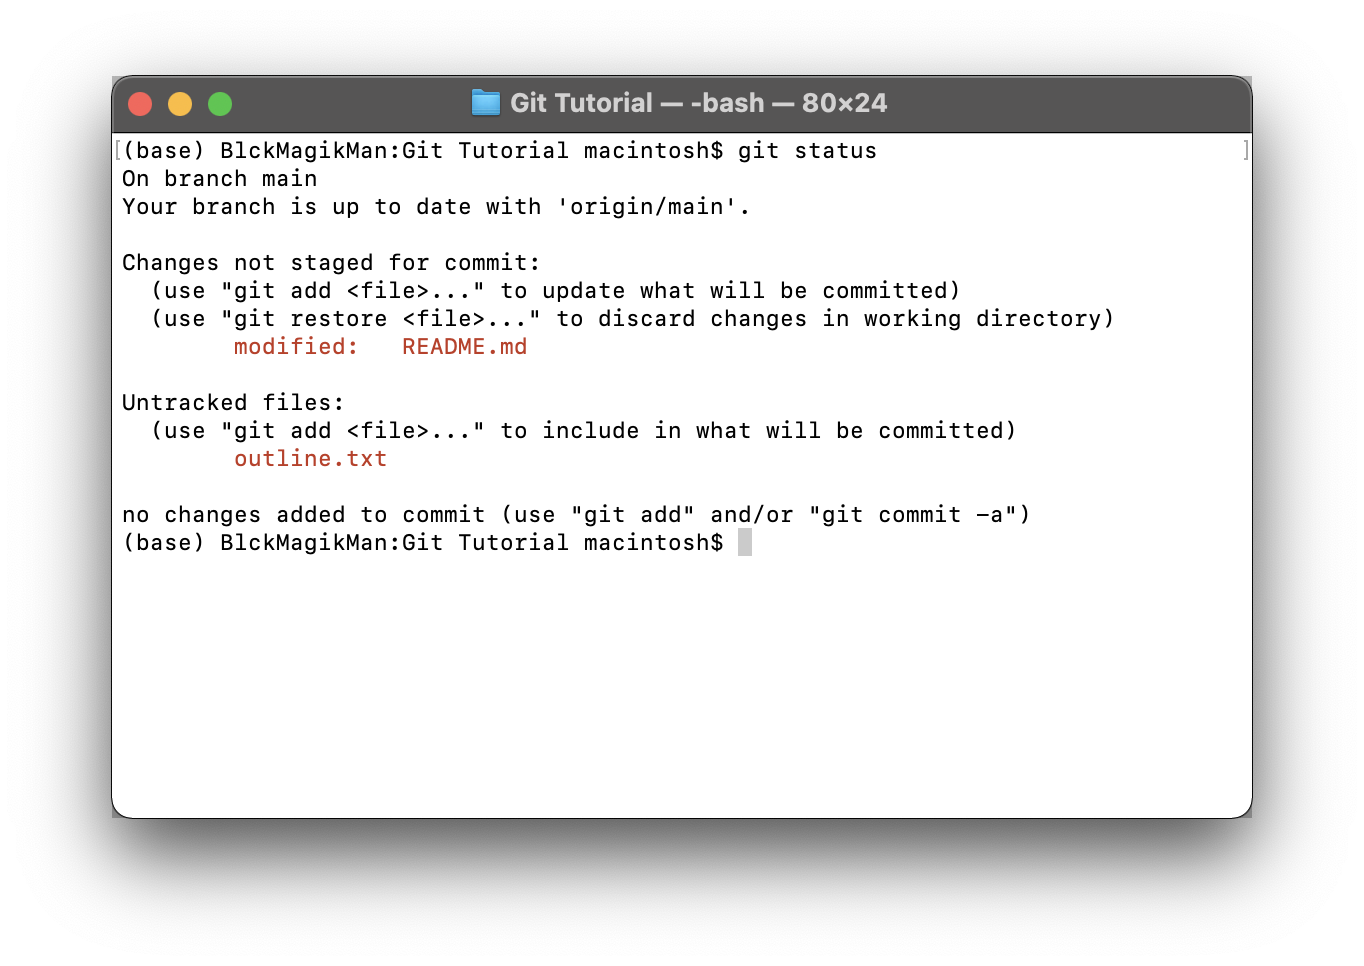
\includegraphics[width=8cm]{shot2.png}
\end{center}

Now let's commit and push our file.
\begin{verbatim}
git commit -m "adding to README"
git push
\end{verbatim}

\section{Stashing and Branching}

Now let's say that we wanted to add a new feature to our project. 
It is better to reserve finished items on the main branch so that if more than one person is working on it they can branch off without having to wait for you to finish. You can think of branching as working on your own copy of the code that will later be added to the main line of code.

\begin{center}
    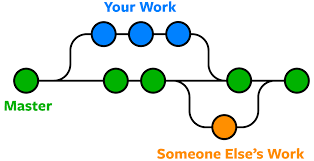
\includegraphics[width=8cm]{shot3.png}
\end{center}

In order to branch we have to create one and then switch to it. Currently, we should have untracked changes to outline.txt so in order to switch branches without deleting those changes, we need to stash them. First, the changes need to be tracked in order to stash them then we can use the "git stash" command to stash the changes to outline.txt. Now to check that our file has been stashed we can use "git stash list". Now you should have a clean working tree, which can be checked with "git status". To move to another branch we have to create the branch and then check it out:

\begin{verbatim}
    git branch newFeature
    git checkout newFeature
\end{verbatim}
or use the shortcut
\begin{verbatim}
    git checkout -b newFeature
\end{verbatim}

Here lets create a python file that is going to represent our new feature.

\begin{center}
    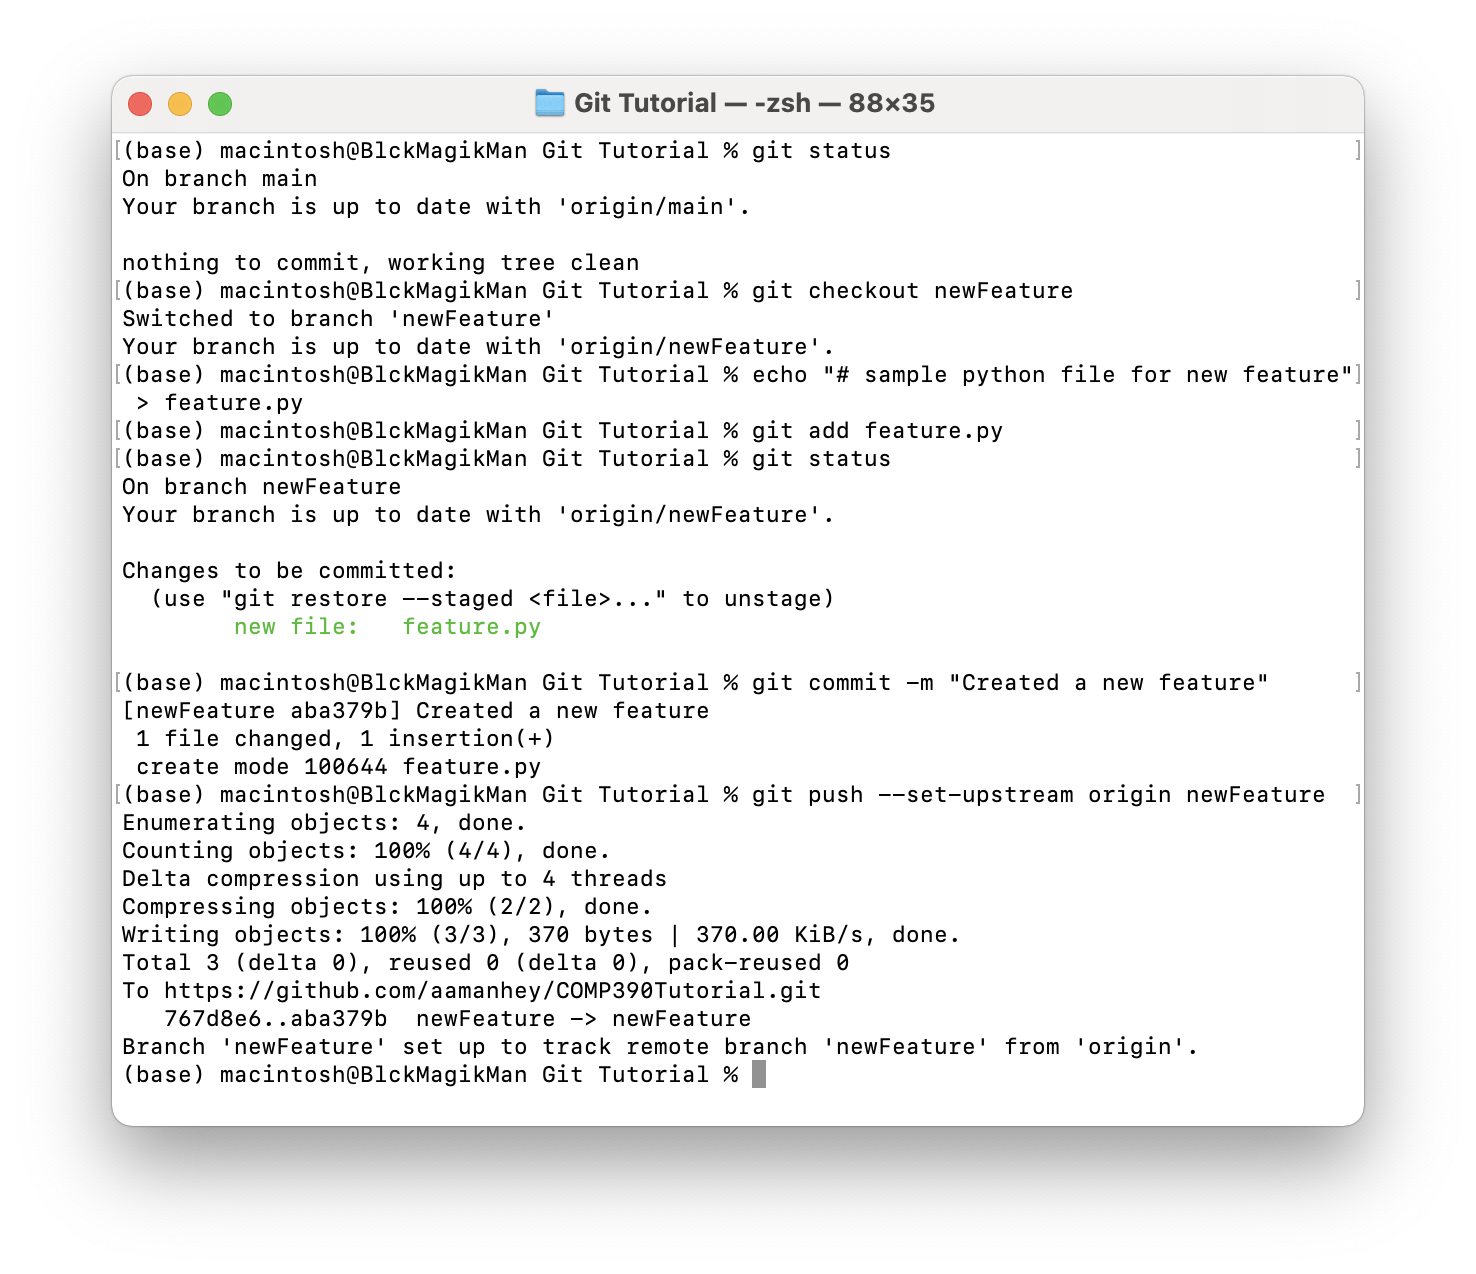
\includegraphics[width=8cm]{newFeature.png}
\end{center}

Now that we've created the new feature let's go back to the main branch and merge the newFeature branch. This lets you take the independent paths of development created by the branches and combine them into a single branch, effectively bringing the changes we made on the newFeature branch onto the main branch.

\begin{verbatim}
    git checkout main
    git merge newFeature
\end{verbatim}

If we were to continue to develop the new feature we could keep the newFeature branch but in this case, let's delete it:

\begin{verbatim}
    git branch -d newFeature
\end{verbatim}

Now to bring back our stashed changes we can use the the \textbf{git stash apply} command to bring back the changes that were last stashed. It would be good practice to unstash our outline and then push those changes but it is not necessary for this tutorial. Since we've pushed a change from a branch other than main, newFeature, we need to create a pull request on GitHub to finalize the incorporation of our changes.

\newpage
\section{Pull Requests}
This part of the tutorial will show you how to make pull requests on GitHub.
Open up your repository on GitHub. You should see a notification that recent pushes have been made to the main branch (Figure 1).

\begin{figure}
    \centering
    \begin{minipage}{0.45\textwidth}
        \centering
        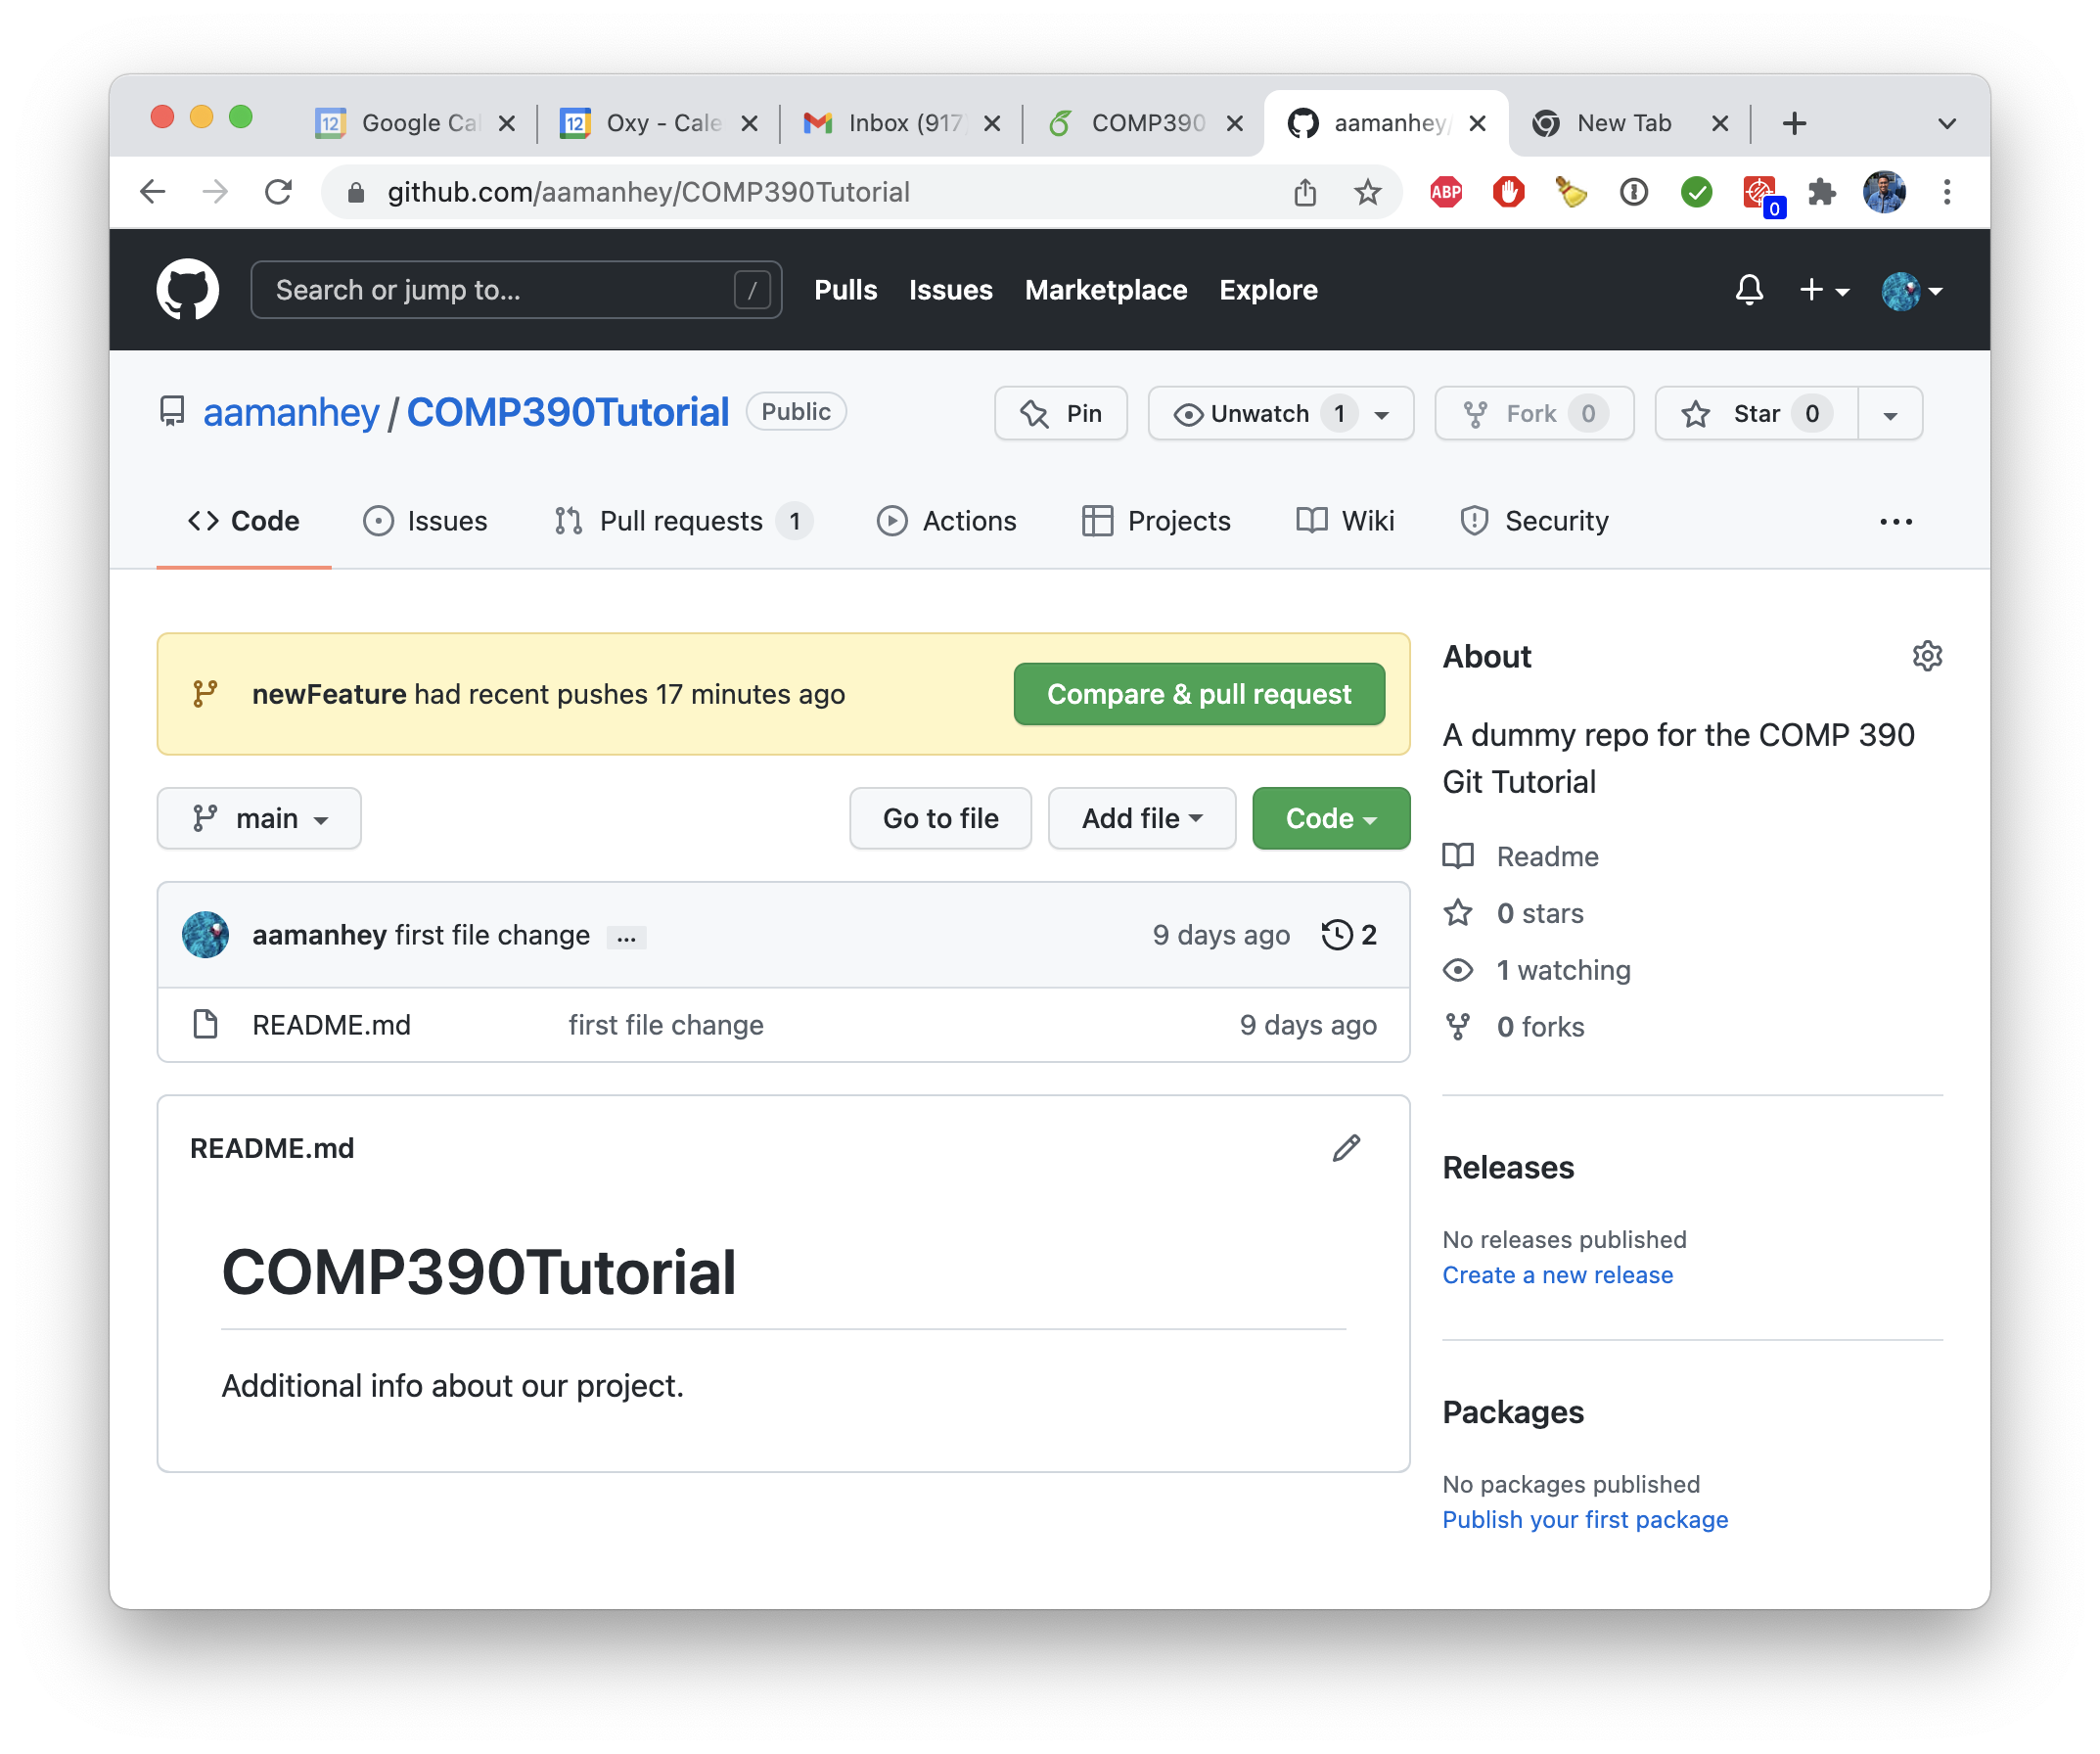
\includegraphics[width=6cm]{pr1.png}
        \caption{Push Notification}
    \end{minipage}\hfill
    \begin{minipage}{0.45\textwidth}
        \centering
        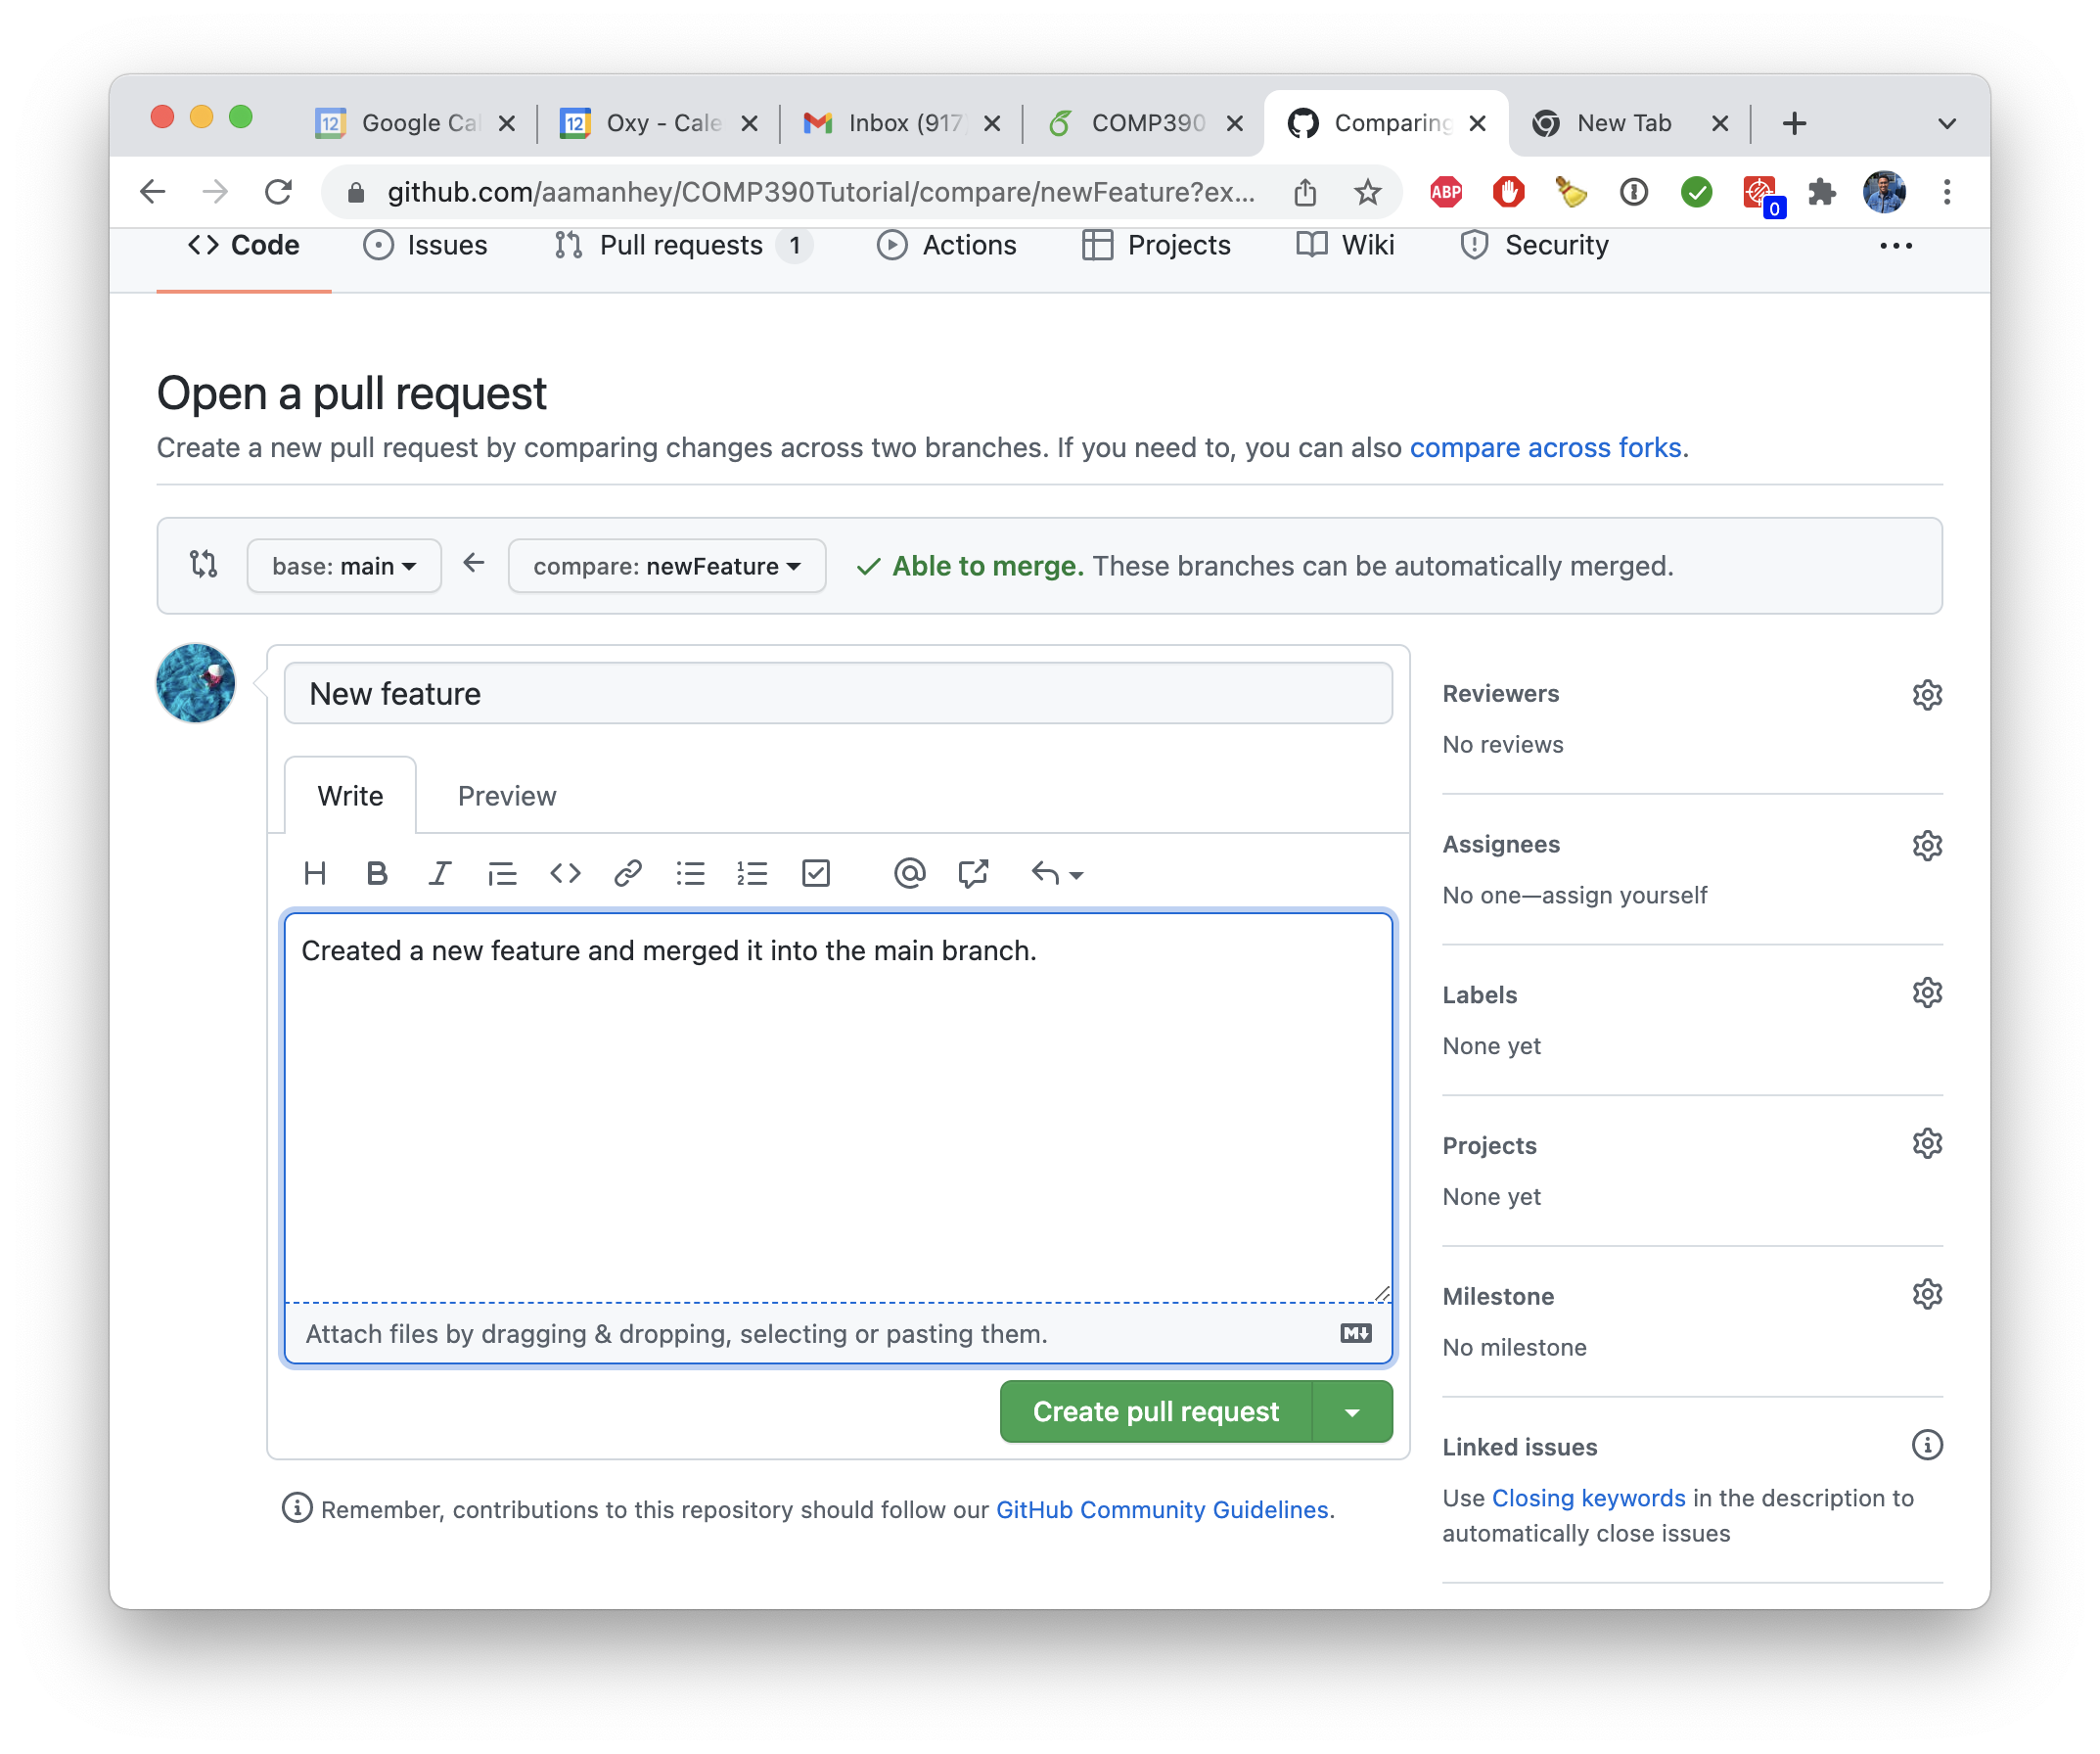
\includegraphics[width=6cm]{pr2.png}
        \caption{Open Pull Request}
    \end{minipage}\hfill
    \begin{minipage}{0.45\textwidth}
        \centering
        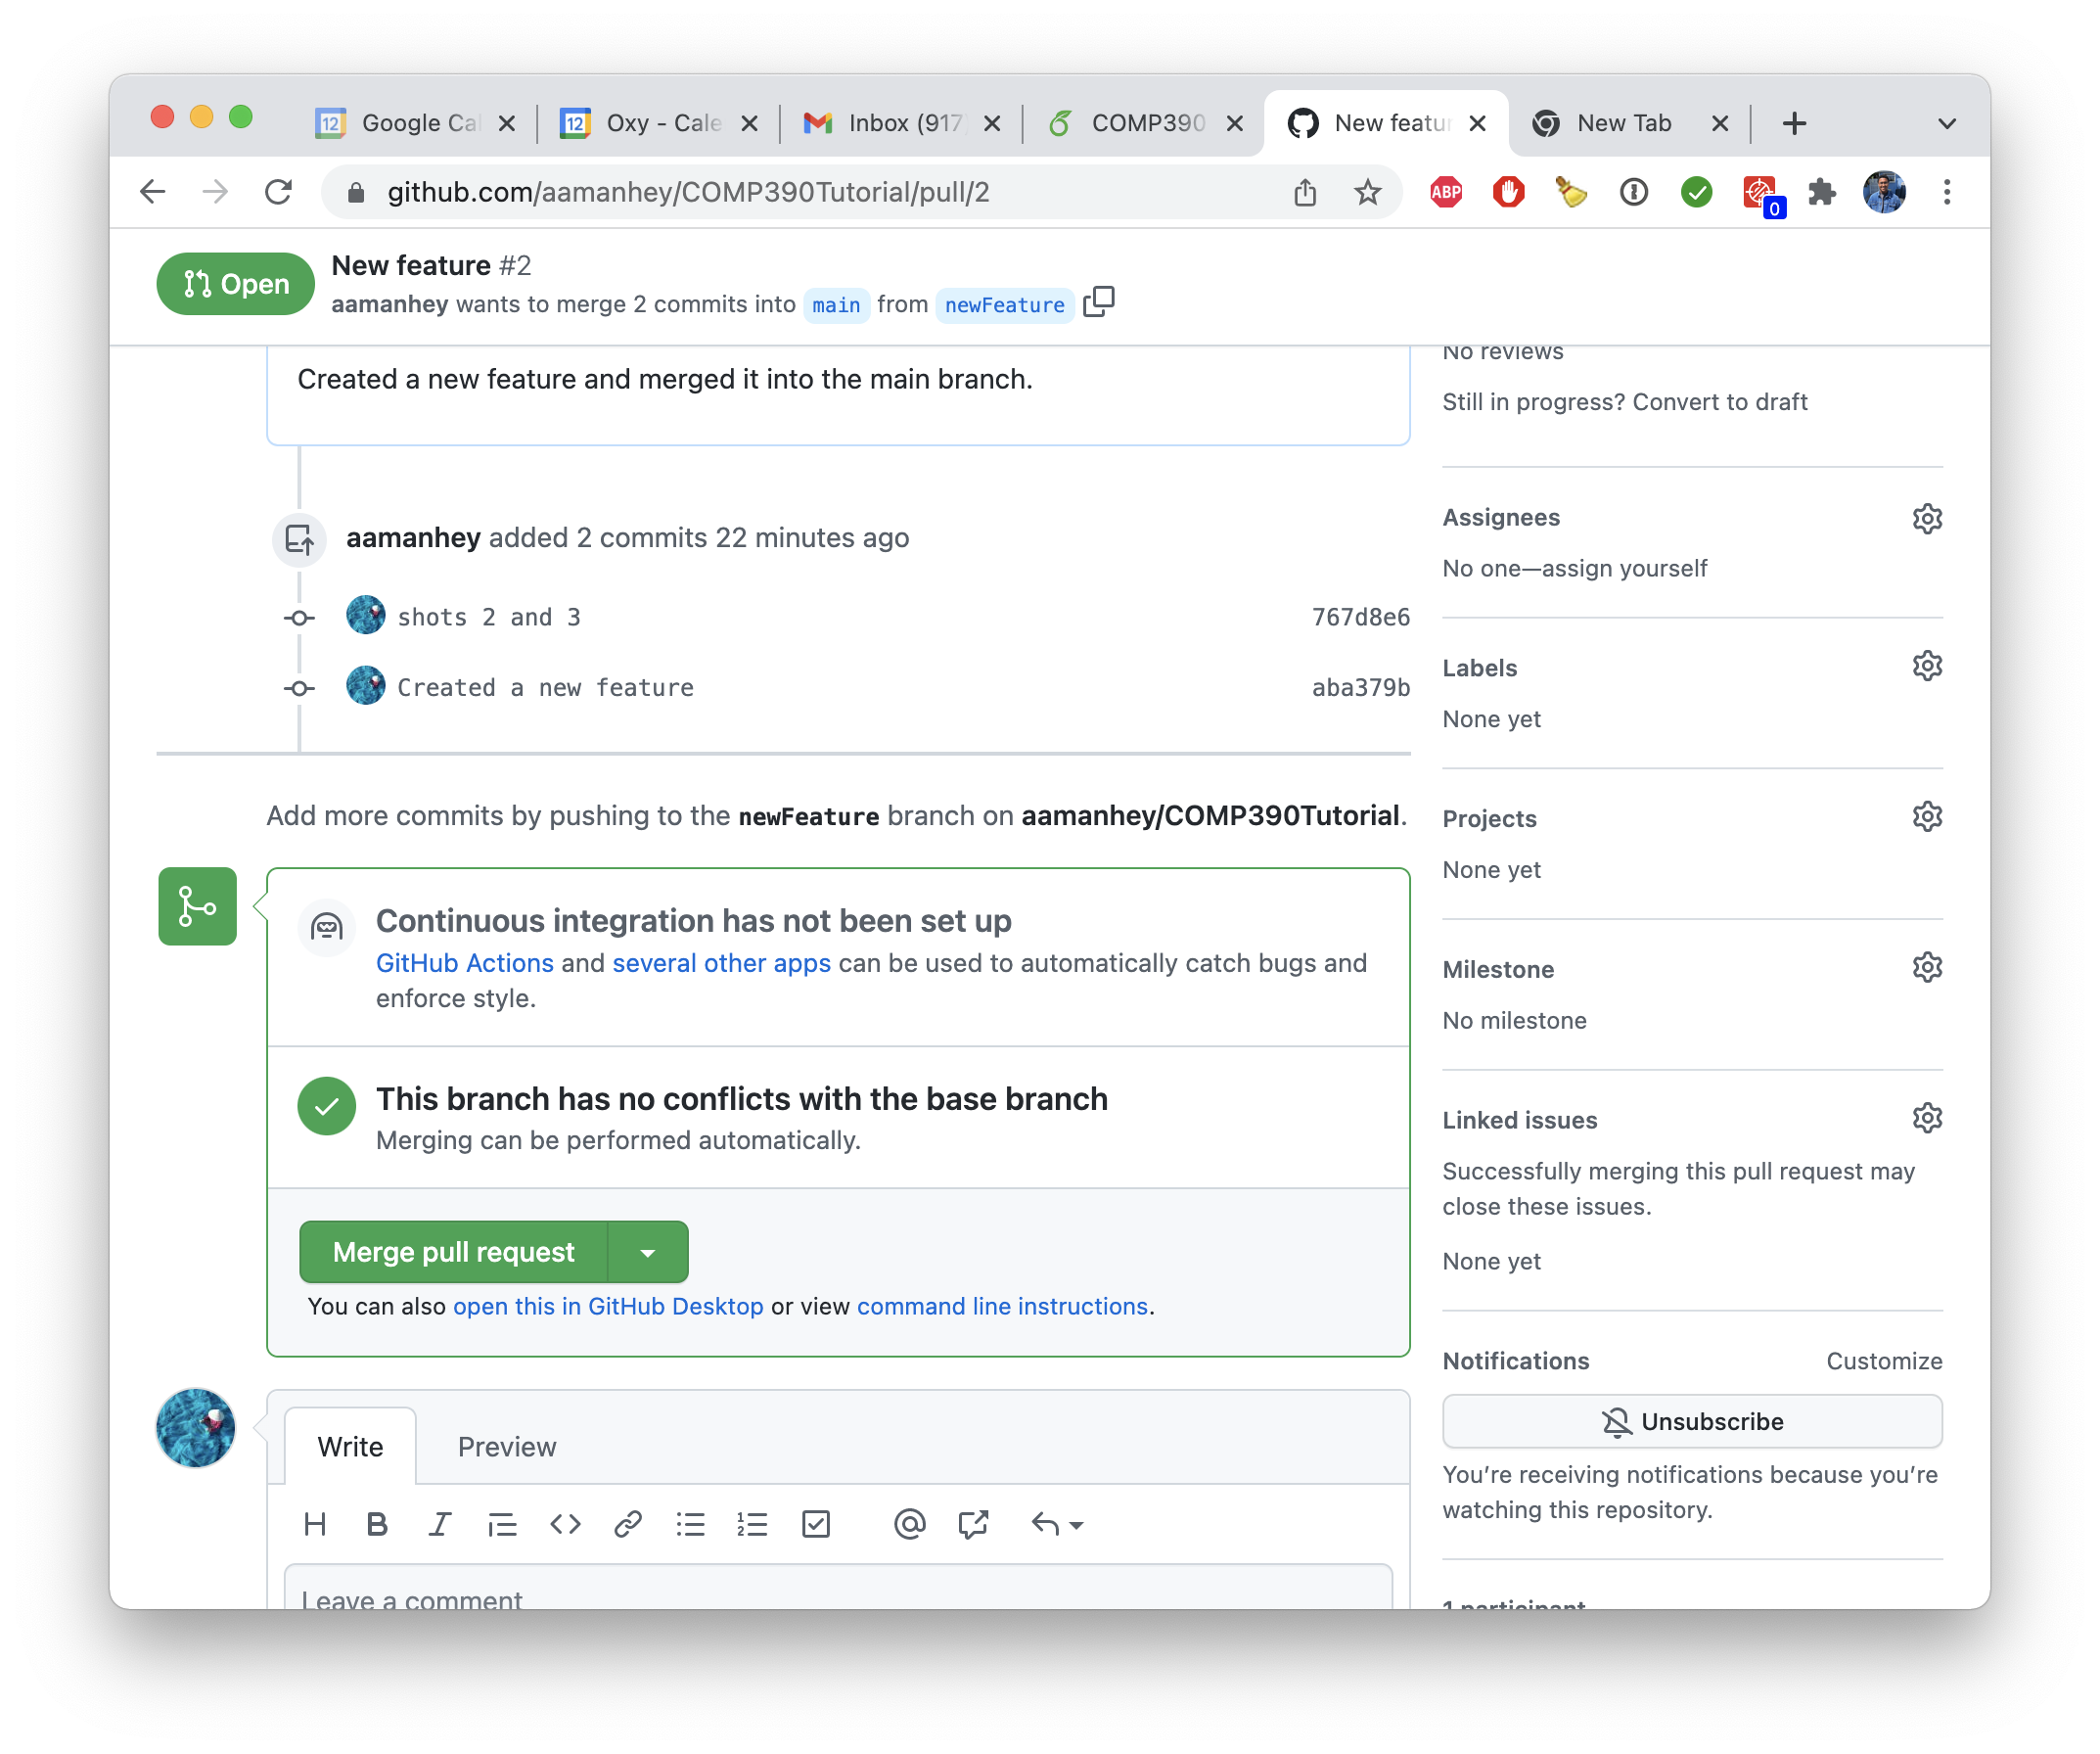
\includegraphics[width=6cm]{pr3.png}
        \caption{Merge Pull Request}
    \end{minipage}\hfill
    \begin{minipage}{0.45\textwidth}
        \centering
        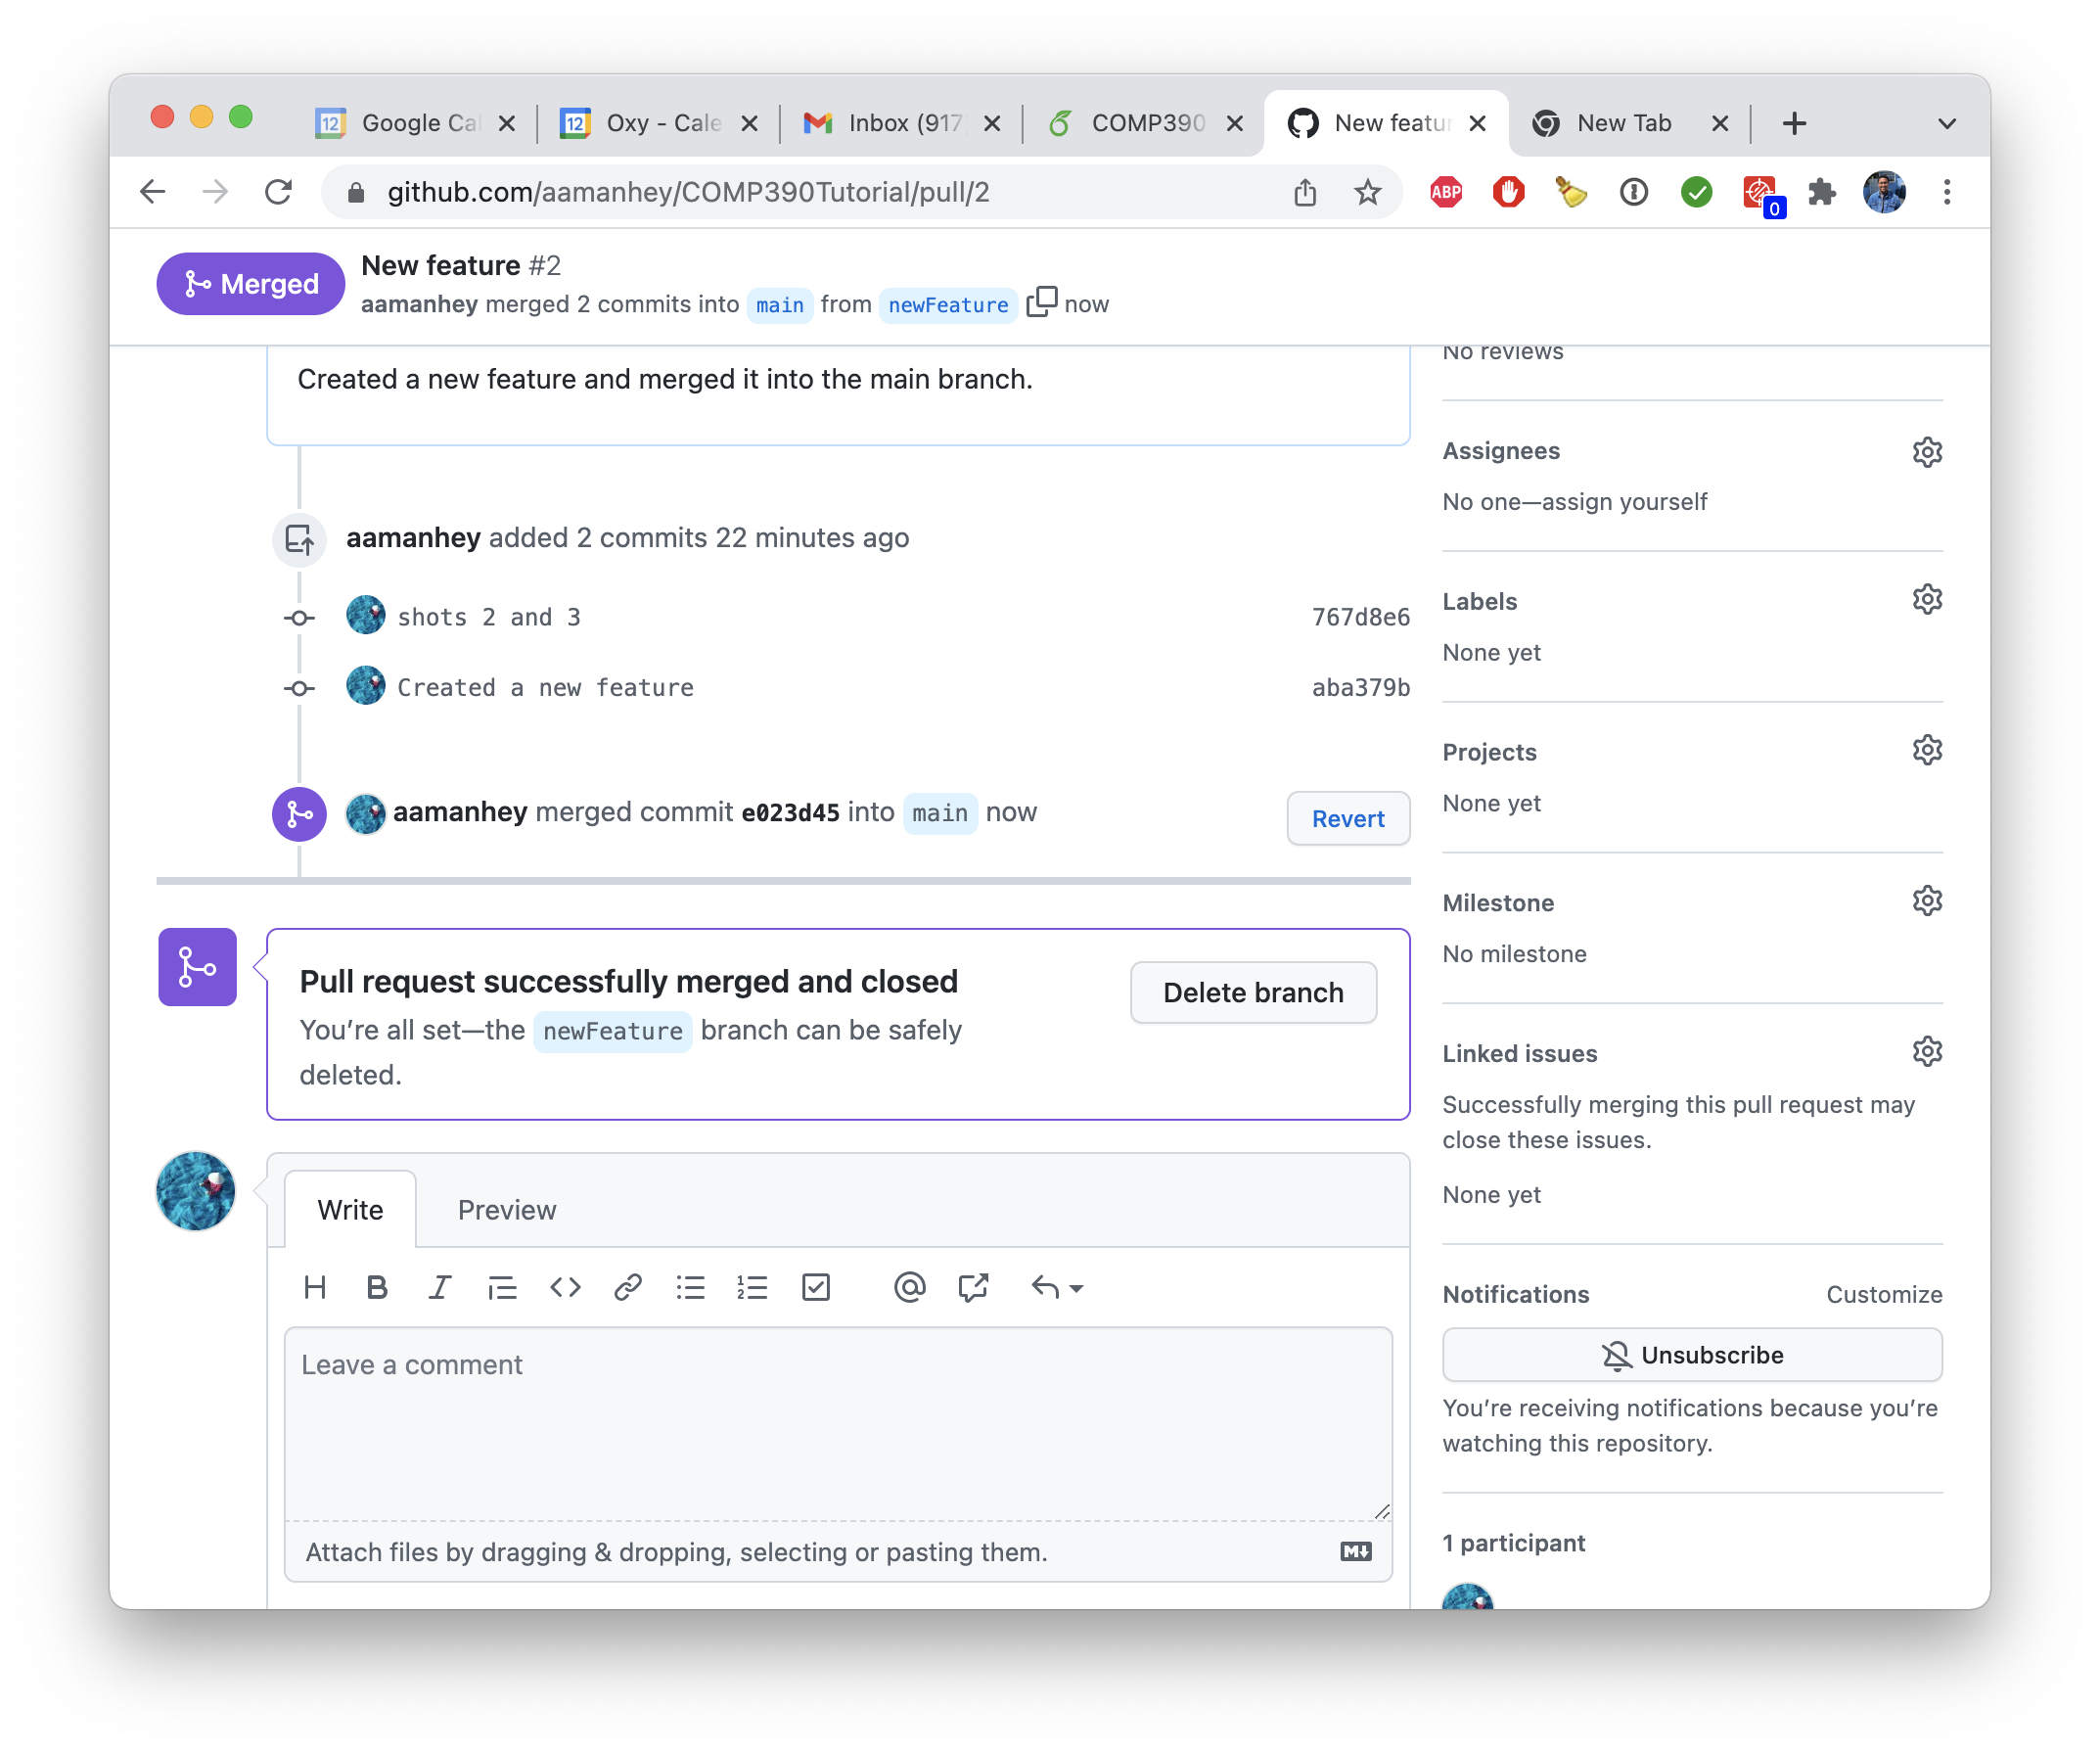
\includegraphics[width=6cm]{pr4.png}
        \caption{Successful Merge}
    \end{minipage}
\end{figure}

If you click on the \textbf{Compare \& pull request} button it should navigate you to an open pull request page where you can add a description of your pull request (Figure 2).
Once you create the pull request you'll be shown all the commits that have been made to that branch before and GitHub will check to see if your code can be merged into the main branch or if a conflict must be handled. You shouldn't see any merge conflicts so you should be able to press \textbf{Merge pull request} (Figure 3).
The page should change and you should now see a message that your pull request was successfully merged (Figure 4).

Now when you go back to your repository's code you should see your feature.py file.

\begin{center}
    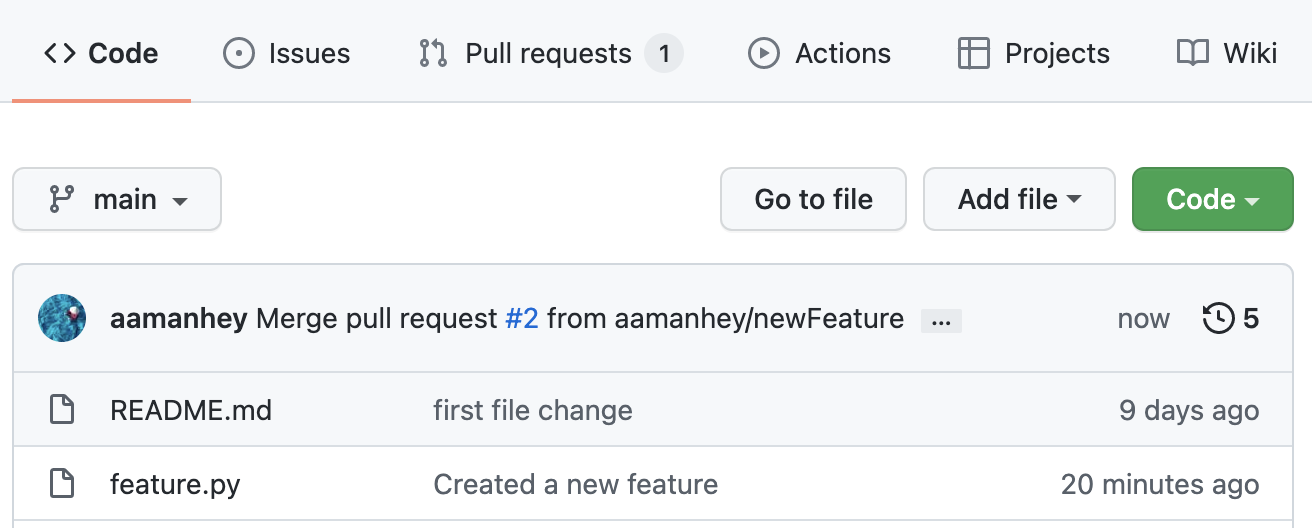
\includegraphics[width=8cm]{pr5.png}
\end{center}

\begin{center}
    Congratulations! You have successfully created a GitHub repository, created and modified file, stashed and unstashed changes, created, used, merged, and deleted branches, and created a pull request!
\end{center}


\end{document}
